\documentclass{standalone}
\usepackage{tikz}
\usetikzlibrary{patterns, positioning}


\begin{document}
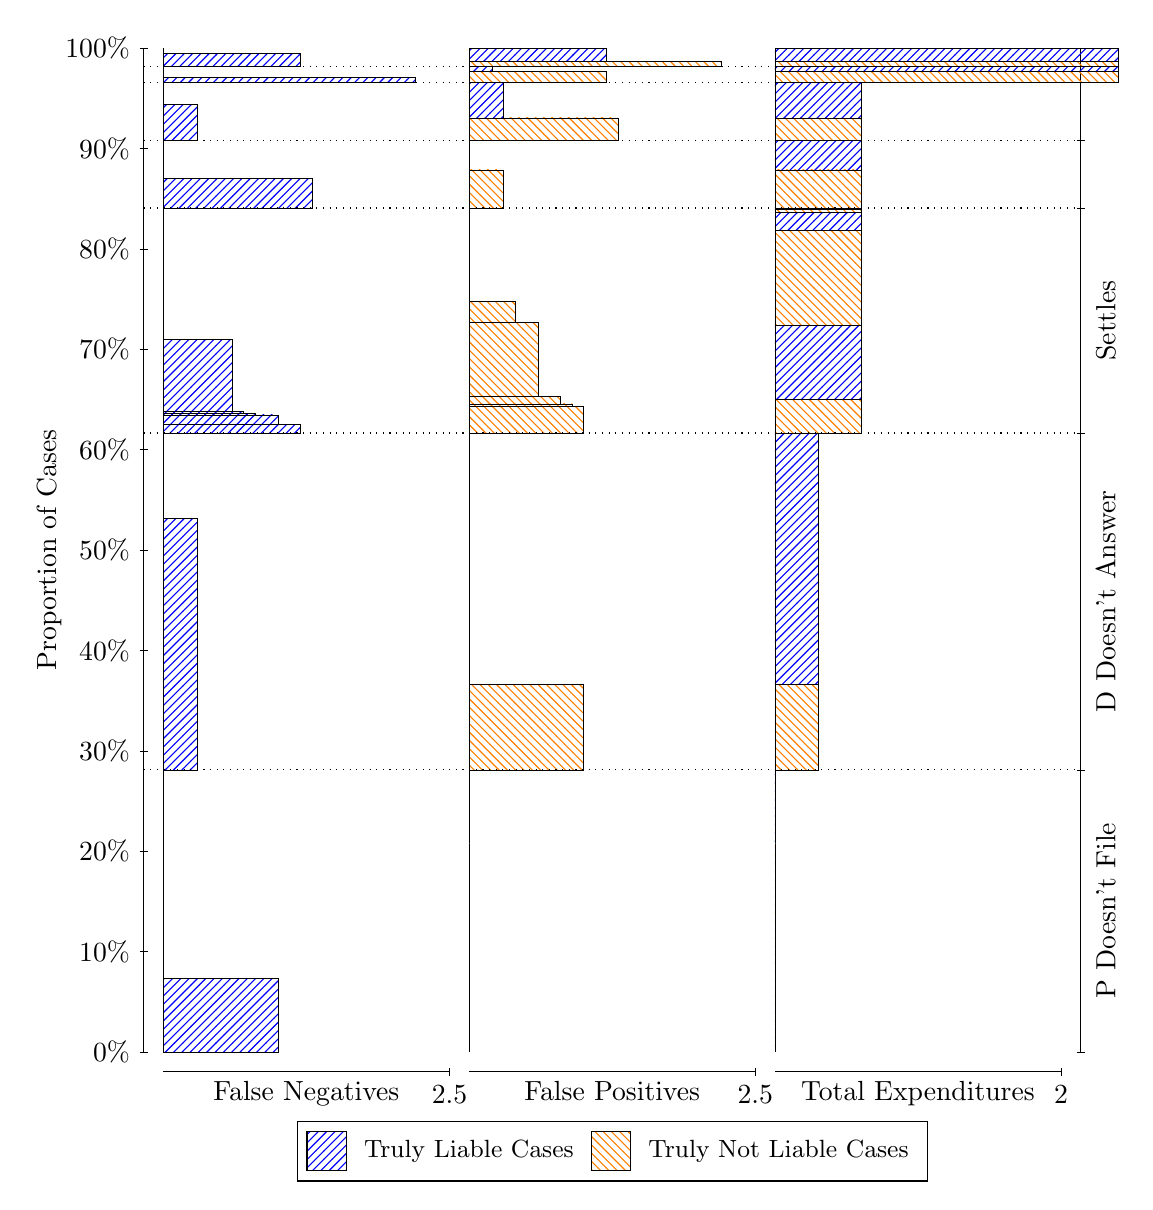
\begin{tikzpicture}
\draw[black, very thin] (1.5,1.75) -- (1.5,14.5);
\node[rotate=90, text=black, anchor=center] at (0.3, 8.125) {Proportion of Cases};
\draw[black, very thin] (1.45,1.75) -- (1.55,1.75);
\node[text=black, anchor=east] at (1.45, 1.75) {0\%};
\draw[black, very thin] (1.45,3.025) -- (1.55,3.025);
\node[text=black, anchor=east] at (1.45, 3.025) {10\%};
\draw[black, very thin] (1.45,4.3) -- (1.55,4.3);
\node[text=black, anchor=east] at (1.45, 4.3) {20\%};
\draw[black, very thin] (1.45,5.575) -- (1.55,5.575);
\node[text=black, anchor=east] at (1.45, 5.575) {30\%};
\draw[black, very thin] (1.45,6.85) -- (1.55,6.85);
\node[text=black, anchor=east] at (1.45, 6.85) {40\%};
\draw[black, very thin] (1.45,8.125) -- (1.55,8.125);
\node[text=black, anchor=east] at (1.45, 8.125) {50\%};
\draw[black, very thin] (1.45,9.4) -- (1.55,9.4);
\node[text=black, anchor=east] at (1.45, 9.4) {60\%};
\draw[black, very thin] (1.45,10.675) -- (1.55,10.675);
\node[text=black, anchor=east] at (1.45, 10.675) {70\%};
\draw[black, very thin] (1.45,11.95) -- (1.55,11.95);
\node[text=black, anchor=east] at (1.45, 11.95) {80\%};
\draw[black, very thin] (1.45,13.225) -- (1.55,13.225);
\node[text=black, anchor=east] at (1.45, 13.225) {90\%};
\draw[black, very thin] (1.45,14.5) -- (1.55,14.5);
\node[text=black, anchor=east] at (1.45, 14.5) {100\%};

\draw[black, very thin] (13.4,1.75) -- (13.4,14.5);
\draw[black, very thin] (13.35,1.75) -- (13.45,1.75);
\node[anchor=west] at (13.35, 1.75) {};
\draw[black, very thin] (13.35,5.3339) -- (13.45,5.3339);
\node[anchor=west] at (13.35, 5.3339) {};
\draw[black, very thin] (13.35,9.6109) -- (13.45,9.6109);
\node[anchor=west] at (13.35, 9.6109) {};
\draw[black, very thin] (13.35,12.468) -- (13.45,12.468);
\node[anchor=west] at (13.35, 12.468) {};
\draw[black, very thin] (13.35,13.328) -- (13.45,13.328);
\node[anchor=west] at (13.35, 13.328) {};
\draw[black, very thin] (13.35,14.067) -- (13.45,14.067);
\node[anchor=west] at (13.35, 14.067) {};
\draw[black, very thin] (13.35,14.265) -- (13.45,14.265);
\node[anchor=west] at (13.35, 14.265) {};
\draw[black, very thin] (13.35,14.5) -- (13.45,14.5);
\node[anchor=west] at (13.35, 14.5) {};

\draw[black, very thin, pattern color=blue, pattern=north east lines] (1.75,1.75) rectangle (3.2033,2.6848);
\draw[black, very thin, pattern color=orange, pattern=north west lines] (1.75,2.6848) rectangle (1.75,5.3339);
\draw[black, very thin, pattern color=blue, pattern=north east lines] (1.75,5.3339) rectangle (2.186,8.522);
\draw[black, very thin, pattern color=orange, pattern=north west lines] (1.75,8.522) rectangle (1.75,9.6109);
\draw[black, very thin, pattern color=blue, pattern=north east lines] (1.75,9.6109) rectangle (3.494,9.7215);
\draw[black, very thin, pattern color=blue, pattern=north east lines] (1.75,9.7215) rectangle (3.2033,9.8401);
\draw[black, very thin, pattern color=blue, pattern=north east lines] (1.75,9.8401) rectangle (2.9127,9.8629);
\draw[black, very thin, pattern color=blue, pattern=north east lines] (1.75,9.8629) rectangle (2.7673,9.8821);
\draw[black, very thin, pattern color=blue, pattern=north east lines] (1.75,9.8821) rectangle (2.622,10.799);
\draw[black, very thin, pattern color=orange, pattern=north west lines] (1.75,10.799) rectangle (1.75,12.468);
\draw[black, very thin, pattern color=blue, pattern=north east lines] (1.75,12.468) rectangle (3.6393,12.843);
\draw[black, very thin, pattern color=orange, pattern=north west lines] (1.75,12.843) rectangle (1.75,13.328);
\draw[black, very thin, pattern color=blue, pattern=north east lines] (1.75,13.328) rectangle (2.186,13.782);
\draw[black, very thin, pattern color=orange, pattern=north west lines] (1.75,13.782) rectangle (1.75,14.067);
\draw[black, very thin, pattern color=blue, pattern=north east lines] (1.75,14.067) rectangle (4.9473,14.131);
\draw[black, very thin, pattern color=orange, pattern=north west lines] (1.75,14.131) rectangle (1.75,14.265);
\draw[black, very thin, pattern color=blue, pattern=north east lines] (1.75,14.265) rectangle (3.494,14.436);
\draw[black, very thin, pattern color=orange, pattern=north west lines] (1.75,14.436) rectangle (1.75,14.5);
\draw[black, very thin, pattern color=orange, pattern=north west lines] (5.6333,1.75) rectangle (5.6333,4.3991);
\draw[black, very thin, pattern color=blue, pattern=north east lines] (5.6333,4.3991) rectangle (5.6333,5.3339);
\draw[black, very thin, pattern color=orange, pattern=north west lines] (5.6333,5.3339) rectangle (7.0867,6.4228);
\draw[black, very thin, pattern color=blue, pattern=north east lines] (5.6333,6.4228) rectangle (5.6333,9.6109);
\draw[black, very thin, pattern color=orange, pattern=north west lines] (5.6333,9.6109) rectangle (7.0867,9.9467);
\draw[black, very thin, pattern color=orange, pattern=north west lines] (5.6333,9.9467) rectangle (6.9413,9.9812);
\draw[black, very thin, pattern color=orange, pattern=north west lines] (5.6333,9.9812) rectangle (6.796,10.076);
\draw[black, very thin, pattern color=orange, pattern=north west lines] (5.6333,10.076) rectangle (6.5053,11.015);
\draw[black, very thin, pattern color=orange, pattern=north west lines] (5.6333,11.015) rectangle (6.2147,11.28);
\draw[black, very thin, pattern color=blue, pattern=north east lines] (5.6333,11.28) rectangle (5.6333,12.468);
\draw[black, very thin, pattern color=orange, pattern=north west lines] (5.6333,12.468) rectangle (6.0693,12.952);
\draw[black, very thin, pattern color=blue, pattern=north east lines] (5.6333,12.952) rectangle (5.6333,13.328);
\draw[black, very thin, pattern color=orange, pattern=north west lines] (5.6333,13.328) rectangle (7.5227,13.613);
\draw[black, very thin, pattern color=blue, pattern=north east lines] (5.6333,13.613) rectangle (6.0693,14.067);
\draw[black, very thin, pattern color=orange, pattern=north west lines] (5.6333,14.067) rectangle (7.3773,14.201);
\draw[black, very thin, pattern color=blue, pattern=north east lines] (5.6333,14.201) rectangle (5.924,14.265);
\draw[black, very thin, pattern color=orange, pattern=north west lines] (5.6333,14.265) rectangle (8.8307,14.329);
\draw[black, very thin, pattern color=blue, pattern=north east lines] (5.6333,14.329) rectangle (7.3773,14.5);
\draw[black, very thin, pattern color=orange, pattern=north west lines] (9.5167,1.75) rectangle (9.5167,4.3991);
\draw[black, very thin, pattern color=blue, pattern=north east lines] (9.5167,4.3991) rectangle (9.5167,5.3339);
\draw[black, very thin, pattern color=orange, pattern=north west lines] (9.5167,5.3339) rectangle (10.062,6.4228);
\draw[black, very thin, pattern color=blue, pattern=north east lines] (9.5167,6.4228) rectangle (10.062,9.6109);
\draw[black, very thin, pattern color=orange, pattern=north west lines] (9.5167,9.6109) rectangle (10.607,10.042);
\draw[black, very thin, pattern color=blue, pattern=north east lines] (9.5167,10.042) rectangle (10.607,10.981);
\draw[black, very thin, pattern color=orange, pattern=north west lines] (9.5167,10.981) rectangle (10.607,12.185);
\draw[black, very thin, pattern color=blue, pattern=north east lines] (9.5167,12.185) rectangle (10.607,12.414);
\draw[black, very thin, pattern color=orange, pattern=north west lines] (9.5167,12.414) rectangle (10.607,12.448);
\draw[black, very thin, pattern color=blue, pattern=north east lines] (9.5167,12.448) rectangle (10.607,12.468);
\draw[black, very thin, pattern color=orange, pattern=north west lines] (9.5167,12.468) rectangle (10.607,12.952);
\draw[black, very thin, pattern color=blue, pattern=north east lines] (9.5167,12.952) rectangle (10.607,13.328);
\draw[black, very thin, pattern color=orange, pattern=north west lines] (9.5167,13.328) rectangle (10.607,13.613);
\draw[black, very thin, pattern color=blue, pattern=north east lines] (9.5167,13.613) rectangle (10.607,14.067);
\draw[black, very thin, pattern color=orange, pattern=north west lines] (9.5167,14.067) rectangle (13.877,14.201);
\draw[black, very thin, pattern color=blue, pattern=north east lines] (9.5167,14.201) rectangle (13.877,14.265);
\draw[black, very thin, pattern color=orange, pattern=north west lines] (9.5167,14.265) rectangle (13.877,14.329);
\draw[black, very thin, pattern color=blue, pattern=north east lines] (9.5167,14.329) rectangle (13.877,14.5);
\draw[black, dotted] (1.5,5.3339) -- (13.4,5.3339);
\draw[black, dotted] (1.5,9.6109) -- (13.4,9.6109);
\draw[black, dotted] (1.5,12.468) -- (13.4,12.468);
\draw[black, dotted] (1.5,13.328) -- (13.4,13.328);
\draw[black, dotted] (1.5,14.067) -- (13.4,14.067);
\draw[black, dotted] (1.5,14.265) -- (13.4,14.265);
\draw[black, very thin] (1.75,1.5) -- (5.3833,1.5);
\node[text=black, anchor=north] at (3.5667, 1.5) {False Negatives};
\draw[black, very thin] (5.3833,1.45) -- (5.3833,1.55);
\node[text=black, anchor=north] at (5.3833, 1.45) {2.5};

\draw[black, very thin] (5.6333,1.5) -- (9.2667,1.5);
\node[text=black, anchor=north] at (7.45, 1.5) {False Positives};
\draw[black, very thin] (9.2667,1.45) -- (9.2667,1.55);
\node[text=black, anchor=north] at (9.2667, 1.45) {2.5};

\draw[black, very thin] (9.5167,1.5) -- (13.15,1.5);
\node[text=black, anchor=north] at (11.333, 1.5) {Total Expenditures};
\draw[black, very thin] (13.15,1.45) -- (13.15,1.55);
\node[text=black, anchor=north] at (13.15, 1.45) {2};

\node[text=black, centered, rotate=90] at (13.72, 3.5419) {P Doesn't File};
\node[text=black, centered, rotate=90] at (13.72, 7.4724) {D Doesn't Answer};
\node[text=black, centered, rotate=90] at (13.72, 11.039) {Settles};





\draw (7.449999999999999,1.5) node[draw=none] (baseCoordinate) {};
\begin{scope}[align=center]
        \matrix[scale=0.5, draw=black, below=0.5cm of baseCoordinate, nodes={draw}, column sep=0.1cm]{
            \node[rectangle, draw, minimum width=0.5cm, minimum height=0.5cm, pattern color=blue, pattern=north east lines] {}; &
            \node[draw=none, font=\small, text=black] (B) {Truly Liable Cases}; &
            \node[rectangle, draw, minimum width=0.5cm, minimum height=0.5cm, pattern color=orange, pattern=north west lines] {}; &
            \node[draw=none, font=\small, text=black] (B) {Truly Not Liable Cases}; \\
            };
\end{scope}

\end{tikzpicture}
\end{document}